%
% elnino.tex
%
% (c) 2018 Prof Dr Andreas Müller, Hochschule Rapperswil
%
\chapter{El Niño Southern Oscillation\label{chapter:elnino}}
\lhead{Kapitel \thechapter: El Niño Southern Oscillation}
Die Klimaentwicklung hängt wesentlich davon ab, wie Energie an der
Erdoberfläche verteilt wird.
Aus diesem Grund haben wir in Kapitel~\ref{chapter:fluiddynamik}
die Strömungsdynamik als den wesentlichen Mechanismus des 
Energietransportes in der Atmoshpäre studiert.
Und in Kapitel~\ref{chapter:thc} haben wir mit der Modellierung der
thermohalinen Zirkulation eine alternative Möglichkeit kennengelernt,
den Energie-Transport in den Weltmeeren zu beschreiben.

Das El Niño-Phänomen im Pazifik ist ein interessantes Teilsystem des
Klimasystems, welches einigermassen gut isoliert behandelt werden kann.
Die Modellierung, die wir in diesem Kapitel anstreben, braucht
einerseits die Ideen der Fluiddynamik, um die Energietransportmechanismen
zu beschreiben, und andererseits die Idee der Box-Modelle, um aus diesen
Mechanismen eine einfache gewöhnliche Differentiagleichung abzuleiten,
mit deren Hilfe die Dynamik des El~Niño studiert werden kann.
\index{El Niño}%
\index{ENSO}%

%
% elnino.tex
%
% (c) 2018 Prof Dr Andreas Müller, Hochschule Rapperswil
%
\chapter{El Niño Southern Oscillation}
\lhead{El Niño Southern Oscillation}
Die Klimaentwicklung hängt wesentlich davon ab, wie Energie an der
Erdoberfläche verteilt wird.
Aus diesem Grund haben wir in Kapitel~\ref{chapter:fluiddynamik}
die Strömungsdynamik als den wesentlichen Mechanismus des 
Energietransportes in der Atmoshpäre studiert.
Und in Kapitel~\ref{chapter:thc} haben wir mit der Modellierung der
thermohalinen Zirkulation eine alternative Möglichkeit kennengelernt,
den Energie-Transport in den Weltmeeren zu beschreiben.

Das El Niño-Phänomen im Pazifik ist ein interessantes Teilsystem des
Klimasystems, welches einigermassen gut als isoliertes Teilsystem 
behandelt werden kann.
Die Modellierung, die wir in diesem Kapitel anstreben, braucht
einerseits die Ideen der Fluiddynamik, um die Energietransportmechanismen
zu beschreiben, und andererseits die Idee der Box-Modelle, um aus diesen
Mechanismen eine einfache gewöhnliche Differentiagleichung abzuleiten,
mit deren Hilfe die Dynamik des El~Niño studiert werden kann.

\section{El Niño}
\rhead{El Niño}

%
% kelvin.tex
%
% (c) 2018 Prof Dr Andreas Müller, Hochschule Rapperswil
%
\section{Kelvin-Wellen\label{section:elnino:kelvin}}
\rhead{Kelvin-Wellen}
In diesem Abschnitt soll die Ausbreitung von Anomalien in der Höhe
der Meeresoberfläche in der Nähe des Äquators studiert werden.

\subsection{Kelvin-Wellen\label{subsection:kelvin}}
\index{Kelvin-Wellen}
In der einfachsten Form führt ein Tiefdruckgebiet über dem zentralen
Pazifik dazu, dass die Meeresoberfläche über die Normalhöhe ansteigt.
Wenn sich das Tiefdruckgebiet auffüllt und die Druckkraft zur Aufrechterhaltung
dieser Anomalie wegfällt, wird dieser ``Wasserberg'' zerfallen.
Mit Hilfe der Gleichungen der Strömungsdynamik sollte sich die Ausbreitung
dieser Wellen beschreiben lassen.

Da die Anfangsbedingungen symmetrisch bezüglich einer Spiegelung an
der Äquatorebene sind, dürfen wir annehmen, dass auch die resultierende
Strömung diese Symmetrie hat.
In unmittelbarer Nähe des Äquators brauchen wir die Krümmung der
Erdoberfläche nicht zu berücksichtigen, und können daher mit einem
$x$-$y$-Koordinatensystem arbeiten, in dem $x$ die Richtung entlang des
Äquators und $y$ die Richtung entlang der Längenkreise ist (siehe auch
die Beschreibung der $\beta$-Ebene auf
Seite~\pageref{skript:betaplane:definition}).
\index{$\beta$-Ebene}%
Die Strömungsgeschwindigkeitskomponenten nennen wir $u$ entlang des
Äquators und $v$ entlang der Längenkreise.
Die Anomalie der Höhe der Meeresoberfläche bezeichnen wir mit $h(x,y)$.

\subsection{Bewegungsgleichung für Kelvin-Wellen}
Die zeitliche Änderung der Geschwindigkeit, also die Beschleunigung,
ist nach dem zweiten Newtonschen Gesetz proportional zu den Kräften.
Die Schwerkraft versucht, den Wasserberg abzubauen.
Wasser wird in diejenige Richtung beschleunigt, in die die Höhe $h(x,y)$
abnimmt.
Ausserdem wirkt die Coriolis-Kraft, die die Strömung auf der Nordhalbkugel
nach rechts ablenkt und auf der Südhalbkugel nach links.
So erhalten wir die Bewegungsgleichungen
\begin{equation}
\begin{aligned}
\frac{\partial u}{\partial t}
&=
\phantom{-}
fv - g\frac{\partial h}{\partial x}
\\
\frac{\partial v}{\partial t}
&=
-fu - g\frac{\partial h}{\partial y}.
\end{aligned}
\label{elnino:kelvin:newton}
\end{equation}
Dies ist ein System von zwei partiellen Differentialgleichung für 
drei unbekannte Funktionen $h$, $u$ und $v$, es ist also mindestens
noch eine weitere Gleichung nötig, damit das Problem überhaupt gelöst
werden kann.

Abfliessendes Wasser reduziert die Höhenanomalie.
Die Kontinuitätsgleichung~\eqref{skript:kontinuitaetsgleichung}
besagt, dass die Abnahme der Höhenanomalie $h$ proportional ist zur
Divergenz des Geschwindigkeitsfeldes.
Die fehlende Differentialgleichung ist daher
\begin{equation}
\frac{\partial h}{\partial t}
=
-H\biggl(
\frac{\partial u}{\partial x} + \frac{\partial v}{\partial y}
\biggr).
\label{elnino:kelvin:kont}
\end{equation}
Gesucht ist jetzt also eine Lösung der Differentialgleichungen
\eqref{elnino:kelvin:newton} und \eqref{elnino:kelvin:kont}.

\subsection{Wellengleichung}
Wir interessieren uns nur für eine Lösung in unmittelbarer Nähe des
Äquators und dürfen daher annehmen, dass sich das Wasser nicht
entlang der Längenkreise bewegt, dass also $v=0$ gilt.
Die Differentialgleichungen
\eqref{elnino:kelvin:newton} und \eqref{elnino:kelvin:kont}
vereinfachen sich damit zu
\begin{align}
\frac{\partial u}{\partial t}
&=
\phantom{-fu}
 - g\frac{\partial h}{\partial x}
\label{kelvin:naeherung:1}
\\
0
&=
-fu - g\frac{\partial h}{\partial y}
\label{kelvin:naeherung:2}
\\
\frac{\partial h}{\partial t}
&=
-H
\frac{\partial u}{\partial x}
\label{kelvin:naeherung:3}
\end{align}
Wir suchen nach einem Wellenphänomen entlang des Äquators, dafür
brauchen wir eine Wellengleichung in den Variablen $t$ und $x$,
die in den Gleichungen \eqref{kelvin:naeherung:1} nach
\eqref{kelvin:naeherung:3} vorkommen.
Aus diesen beiden Gleichungen sollte sich eine Wellengleichung
gewinnen lassen.

Indem wir \eqref{kelvin:naeherung:1} nach $x$ und 
\eqref{kelvin:naeherung:3} nach $t$ ableiten, erhalten wir
\begin{equation}
\left.
\begin{aligned}
\frac{\partial^2 u}{\partial x\,\partial t}
&=
-g\frac{\partial^2h}{\partial x^2}
\\
\frac{\partial^2 h}{\partial t^2}
&=
-H\frac{\partial^2 u}{\partial t\,\partial x}
\end{aligned}
\;
\right\}
\quad
\Rightarrow
\quad
\frac{\partial^2 h}{\partial t^2}
=
gH\frac{\partial^2 h}{\partial x^2}
\label{kelvin:wellengleichung}
\end{equation}
Dies ist die gesuchte Wellengleichung für eine Welle mit
Ausbreitungsgeschwindigkeit $c=\sqrt{gH}$.
Im nächsten Abschnitt bestimmen wir ihre Lösungen.

\subsection{Approximative Lösung der Wellengleichung}
Bis jetzt wurde die zweite Gleichung~\eqref{kelvin:naeherung:2}
nicht verwendet, es wurde eigentlich nur das Verhalten der Welle auf
dem Äquator modelliert.
Da wir jetzt aber wissen, dass mindestens entlang des Äquators die Lösung
eine Welle mit Ausbreitungsgeschwindigkeit $c=\sqrt{gH}$ ist, können
wir versuchen, auch die $y$-Abhängigkeit zu modellieren.

\subsubsection{Dispersionsrelation}
Eine in $x$-Richtung laufende Welle mit Wellenzahl $k$ kann beschrieben werden
als $\cos(kx-\omega t)$.
Die Wellenzahl $k$ ist positiv für eine nach Osten laufende Welle und negativ
für eine nach Westen laufende Welle.
Überall dort, wo $kx-\omega t=0$ ist, befindet sich ein Wellenberg,
die Position dieses Maximums ist also
\[
x=\frac{\omega}{k}\cdot t,
\]
es bewegt sich also mit der Geschwindigkeit $c=\omega/k$.
Dies ist die sogenannte {\em Phasengeschwindigkeit}.
\index{Phasengeschwindigkeit}%

Wir dürfen allerdings nicht davon ausgehen, dass das Verhältnis $\omega/k$
konstant ist, Wellen mit verschiedenen Frequenzen können sich durchaus
mit verschiedenen Geschwindigkeiten ausbreiten.
Ein Glasprisma ist in der Lage, Licht in seine verschiedene Farben
mit verschiedenen Ausbreitungsgeschwindigkeiten im Glas aufzufächern. 
Dieses Phänomen heisst {\em Dispersion} und äussert sich in einem
\index{Dispersion}%
funktionalen Zusammenhang
\[
\omega = \omega(k)
\]
zwischen Wellenzahl $k$ und Frequenz $\omega$, einer {\em Dispersionsrelation}.
\index{Dispersionsrelation}%

Wir suchen also eine Lösung des Gleichungssystems
\eqref{kelvin:naeherung:1}--\eqref{kelvin:naeherung:3}
in der Form
\[
h_k(t,x,y) = \gamma(y)\cdot \cos(kx-\omega t)
\]
zu finden.
Die Funktion $\gamma(y)$ beschreibt das Profil des ``Wasserberges'' 
in der Nähe des Äquators, wir nehmen daher an, dass $\gamma(y)$ für grosse
Werte von $y$ rasch abnimmt.

Einsetzen des Lösungsansatzes $h_k(t,x,y)$ in die
Gleichung~\eqref{kelvin:wellengleichung} liefert
\begin{equation}
\left.
\begin{aligned}
\frac{\partial^2 h_k}{\partial t^2}
&=
- \omega^2 \gamma(y) \cos(kx-\omega t)
=
-\omega^2 h_k(t,x,y)
\\
\frac{\partial^2 h_k}{\partial x^2}
&=
-
k^2
\gamma(y)
\cos (kx-\omega t)
=
-k^2 h_k(t,x,y)
\end{aligned}
\;\right\}
\quad
\Rightarrow
\quad
\omega^2=gHk^2
\quad\text{oder}\quad
\biggl|
\frac{\omega}{k}\biggr|
=\sqrt{gH}=c
\end{equation}
Aus dieser Dispersionsrelation
liest man ab, dass die Phasengeschwindigkeit einer solchen
Welle unabhängig ist von der Frequenz.

\subsubsection{$y$-Abhängigkeit}
Bis jetzt haben wir die Gleichung~\eqref{kelvin:naeherung:2} nicht
verwendet.
Sie erlaubt, $u$ zu berechnen, es gilt
\[
u=-\frac{g}{f}\,\frac{\partial h}{\partial y}
\qquad
\text{oder für $h_k$}
\qquad
u_k=-\frac{g}{f} \gamma'(y) \sin(kx-\omega t).
\]
Setzt man dies in \eqref{kelvin:naeherung:3} ein, erhält man
\begin{equation}
\left.
\begin{aligned}
\frac{\partial h_k}{\partial t}
&=
-\omega
\gamma(y) \cos(kx-\omega t)
\\
\frac{\partial u_k}{\partial x}
&=
k \frac{g}{f}\gamma'(y) \cos(kx-\omega t)
\end{aligned}
\;\right\}
\qquad\Rightarrow\qquad
-\omega
\gamma(y) \cos(kx-\omega t)
=
-H
k \frac{g}{f}\gamma'(y) \cos(kx-\omega t).
\end{equation}
Nach Kürzen gemeinsamer Faktoren und Umstellen folgt
\begin{equation}
\gamma'(y)
=
\gamma(y) \frac{f}{gH}\frac{\omega}{k}
=
\pm
\frac{f}{c} \gamma(y).
\label{kelvin:gamma:dgl1}
\end{equation}
Das Vorzeichen in \eqref{kelvin:gamma:dgl1} hängt vom Vorzeichen der
Wellenzahl $k$ ab, das obere Vorzeichen steht für eine nach Osten
laufende Welle.

Die Coriolis-Kraft $f$ verschwindet am Äquator, in erster Näherung
ist sie proportional zu $y$, wir schreiben daher $f=\beta y$.
Die Differentialgleichung~\eqref{kelvin:gamma:dgl1} wird damit zu
\begin{equation}
\gamma'(y)
=
\pm
\frac{\beta}{c} 
y\gamma(y).
\label{kelvin:gamma:dgl2}
\end{equation}

Für zunehmende $y$ muss $\gamma$ abnehmen, es muss also $\gamma'(y)<0$ sein
für genügend grosse $y$.
Dies ist aber nur möglich für das negative Vorzeichen, und damit nur
für eine nach Osten laufende Welle.
Im Folgenden konzentrieren wir uns daher auf das negative Zeichen
in \eqref{kelvin:gamma:dgl2}.

Um eine Lösung von \eqref{kelvin:gamma:dgl2} zu finden, teilen wir
durch $\gamma(y)$
und verwenden, dass $\gamma'(y)/\gamma(y)$ die Ableitung des
Logarithmus ist:
\begin{equation}
\frac{\gamma'(y)}{\gamma(y)}
=
\frac{d}{dy}\log \gamma(y) = -\frac{\beta}{c} y
\qquad\Rightarrow\qquad
\log\gamma(y) = -\frac{\beta}{2c}y^2
\qquad\Rightarrow\qquad
\gamma(y) = \exp\biggl(
- \frac{\beta}{2c}y^2
\biggr)
\end{equation}
Das $y$-Profil der Welle ist also eine Gauss-Funktion.
Die Zone, in der sich eine Kelvin-Welle ausbreiten kann, 
wird schmaler, wenn $\beta$ grösser wird, wenn also die 
Rotationsgeschwindigkeit des Planeten grösser wird.
Sie wird kleiner, wenn $c=\sqrt{gH}$ grösser wird, also
bei grösserer Gravitation.


%
% rossby.tex
%
% (c) 2018 Prof Dr Andreas Müller, Hochschule Rapperswil
%

\section{Rossby-Wellen\label{section:elnino:rossby}}
\rhead{Rossby-Wellen}
In der Untersuchung der Kelvin-Wellen haben wir angenommen, dass die
Geschwindigkeit $v$ entlang der Längenkreise verschwindet.
Die Strömung wird aber im Allgemeinen nicht parallel zum Äquator sein.
Wir beobachten zum Beispiel, dass die Westwindströmung 
zwischen verschiedenen geographischen Breiten mäandriert.
Woher kommt diese Wellenbewegung?
\index{Rossby-Wellen}%

\subsection{Zirkulation\label{subsection:rossby:zirkulation}}
Aus der Diskussion der globalen Zirkulation in
Kapitel~\ref{chapter:wetter und klima} wissen wir, dass die
Strömung in Äquatornähe dominiert wird durch eine mittlere
konstante Strömung mit Geschwindigkeit $U$ in Ost-West-Richtung.
Wir suchen daher eine Beschreibung der Abweichungen von dieser
mittleren Strömung.
Unter Verwendung der gleichen Notation wie im
Abschnitt~\ref{section:elnino:kelvin} schreiben wir daher
\[
u'=U+u,\qquad v'=v\qquad\text{mit $u,v\ll U$}.
\]
Die Geschwindigkeitskomponenten $u$ und $v$ sind die Anomalien relativ
zur vorherrschenden mittleren Strömung.

Wir nehmen im Folgenden wieder an, dass die Strömung quellenfrei ist.
Dann lässt sich wie früher gezeigt die Strömung mit einer
Strömungsfunktion $\psi$ als
\begin{equation}
u=-\frac{\partial \psi}{\partial y},\qquad
v=\frac{\partial\psi}{\partial x}
\label{skript:rossby:geschwindigkeit}
\end{equation}
beschreiben.

Die gesuchten Wellen sollen Mäander-Form der Strömung erklären,
also Änderungen der Strömungsrichtungen, die natürlich mit
Änderungen des Drehimpulses einhergehen.
Die Drehimpulsdichte in der Strömung ist gegeben durch die Zirkulation
\[
\zeta
=
\frac{\partial v}{\partial x} - \frac{\partial u}{\partial y}
=
\Delta \psi.
\]
Da der Drehimpuls erhalten ist, muss die Zirkulation in einem
Luftpaket abnehmen, wenn es sich auf der Nordhalbkubel nach Norden
bewegt.
Die Quelle dieser Zirkulationsänderung ist die Erddrehung und damit
die Corioliskraft $f$ und der mathematische Ausdruck der Drehimpulserhaltung
ist die Erhaltung der Grösse $\zeta+f$.

\subsection{Bewegungsgleichung\label{subsection:rossby:bewegungsgleichung}}
Die Grösse $\zeta+f$ ist erhalten, daher muss ihre zeitliche Ableitung
\[
\frac{d(\zeta f)}{dt}=0
\]
verschwinden.
Die Coriolis-Kraft
$f$ hängt nur von $y$ ab, aber die Funktion $\zeta$ hängt von allen
drei Variablen $t$, $x$ und $y$ ab.
Wir berechnen die Ableitung mit Hilfe der Kettenregel:
\begin{align*}
0
=
\frac{d(\zeta+f)}{dt}
&=
\frac{\partial\zeta}{\partial t}
+
\frac{\partial\zeta}{\partial x}\cdot \frac{dx}{dt}
+
\frac{\partial(\zeta+f)}{\partial y}\cdot\frac{dy}{dt}
\\
&\simeq
\frac{\partial\zeta}{\partial t}
+
(U+u)\frac{\partial\zeta}{\partial x}
+
v\biggl(\frac{\partial\zeta}{\partial y} + \frac{\partial f}{\partial y}\biggr).
\end{align*}
Da $u\ll U$ ist, können wir in erster Näherung $u$ im zweiten Term 
vernachlässigen.
Und da $\partial\zeta/\partial y$ ebenfalls sehr klein ist, können
wir dies im letzten Term im Vergleich zu $\partial f/\partial y$
vernachlässigen.
Schliesslich können wir wie in Abschnitt~\ref{section:elnino:kelvin}
die $\beta$-Ebenen-Approximation verwenden und $\partial f/\partial y$
durch $\beta$ ersetzen.
Schliesslich können wir wieder mit \eqref{skript:rossby:geschwindigkeit}
$v$ als Ableitung von $\psi$ nach $x$ ausdrücken.
Wir erhalten so
\[
0
=
\frac{\partial\zeta}{\partial t}
+
U\frac{\partial\zeta}{\partial x}
+
\beta\frac{\partial\psi}{\partial x}
\]
als Bewegungsgleichung.

Indem wir $\zeta=\Delta \psi$ schreiben, erhalten wir so die 
Bewegungsgleichung
\begin{equation}
\frac{\partial\Delta\psi}{\partial t}
+
U\frac{\partial\Delta\psi}{\partial x}
+
\beta\frac{\partial\psi}{\partial x}
=
0.
\label{rossby:gleichung}
\end{equation}


\subsection{Wellenlösungen\label{subsection:rossby:loesungen}}
Gesucht sind Lösungen der Gleichung~\eqref{rossby:gleichung}
in Form kleiner Abweichungen.
Wir erwarten Wellenlösungen und schreiben sie daher in der Form
\begin{equation}
\psi_{kl}(t,x,y)
=
\cos(kx+ly-\omega t).
\label{rossby:ebenewelle}
\end{equation}
Die Ableitungen, die wir für die Bewegungsgleichung
\eqref{rossby:gleichung} benötigen, sind
\begin{align*}
\frac{\partial}{\partial t} \psi_{kl}(t,x,y)
&=
\omega \sin(kx+ly-\omega t)
\\
\frac{\partial}{\partial x} \psi_{kl}(t,x,y)
&=
-k
\sin(kx+ly-\omega t)
\\
\Delta\psi_{kl}
&=
-(k^2+l^2)\cos(kx+ly-\omega t)=-(k^2+l^2)\psi_{kl}(t,x,y).
\end{align*}
Setzen wir dies in die Differentialgleichung
\eqref{rossby:gleichung}
ein, erhalten wir 
\begin{align*}
0
&=
-
\omega(k^2+l^2) 
\sin(kx+ly-\omega t)
+
Uk(k^2+l^2)
\sin(kx+ly-\omega t)
-
\beta k
\sin(kx+ly-\omega t)
\\
&=
-\bigl((\omega-Uk)(k^2+l^2)+\beta k\bigr)
\sin(kx+ly-\omega t).
\end{align*}
Für eine Lösung muss also die Dispersionsrelation
\[
(\omega -Uk)(k^2+l^2) +\beta k=0
\]
gelten.
Aufgelöst nach $\omega$ ist dies
\begin{align}
\omega(k^2+l^2)
&=
Uk(k^2+l^2) -\beta k
\notag
\\
\Rightarrow\qquad
\omega
&=
Uk
-
\frac{\beta k}{k^2+l^2}.
\label{rossby:dispersion}
\end{align}
Eine Wellenlösung mit Wellenzahlen $k$ und $l$ hat daher 
die Ausbreitungsgeschwindigkeit 
\begin{equation}
c=\frac{\omega}{k} = U-\beta\frac{1}{k^2+l^2}
\label{rossby:phasengeschwindigkeit}
\end{equation}
entlang der $x$-Koordinate.
Da der Nenner immer positiv ist, ist $c$ kleiner als $U$, solche
Wellen können sich immer nur in West-Ost-Richtung ausbreiten.

\subsection{Gruppengeschwindigkeit}
Die Phasengeschwindigkeit~\eqref{rossby:phasengeschwindigkeit}
hilft uns nicht, die Dynamik des El Niño zu verstehen, da wir dazu
den Transport von Energie verstehen müssen.
Die ebenen Wellen der Form~\eqref{rossby:ebenewelle} beschreiben eine Welle,
die überall die gleiche Amplitude hat.
Ein Transport von potentieller Energie findet aber nur statt, wenn ein
``Wellenberg'' sich an einen anderen Ort bewegt.
Im Beispiel des ``Wasserberges'' in der Untersuchung zu den Kelvin-Wellen
wird potentielle Energie dadurch transportiert, dass das Wasser des Berges
abfliesst.
Wir müssen daher erst einen ``Wasserberg'' als Überlagerung von 
ebenen Wellen formulieren und dann die zeitliche Entwicklung dieser
Überlagerung studieren.

\subsubsection{Überlagerungen}
Wir gehen von einer eindimensionalen Situation aus und studieren
eine Überlagerung $u(x,t)$ von Wellen der Form $\cos(kx-\omega(k) t)$
mit verschiedenen Wellenzahlen $k$.
Mit der wellenzahlabhängigen Amplitude $\hat f(k)$, dem Spektrum
wie in Kapitel~\ref{chapter:fourier} studiert, lässt sich die
Überlagerung als
\begin{equation}
u(x,t)
=
\int_{-\infty}^\infty \hat f(k)\,\cos(kx-\omega(k)t)\,dk
\label{rossby:reelleueberlagerung}
\end{equation}
schreiben.
Die Bewegung eines solchen Wellenpaketes kann man zum Beispiel
dadurch studieren, dass man die Bewegung des Maximums dieses 
Wellenpaketes verfolgt.
\index{Wellenpaket}

Die Darstellung~\eqref{rossby:reelleueberlagerung} ist für diese
Untersuchung sehr unhandlich, die Rechnungen sind zu umständlich.
Wir schreiben die Wellen daher als Realteil einer komplexen
Welle $e^{i(kx-\omega(k)t)}$, also
\begin{equation}
u(x,t)
=
\operatorname{Re}
\int_{-\infty}^\infty \hat f(k)\,e^{i(kx-\omega(k)t)}\,dk.
\label{rossby:komplexeueberlagerung}
\end{equation}
Dabei lassen wir auch zu, dass $\hat{f}(k)$ komplexe Werte annimmt.

\subsubsection{Wellenpakete}
\begin{figure}
\centering
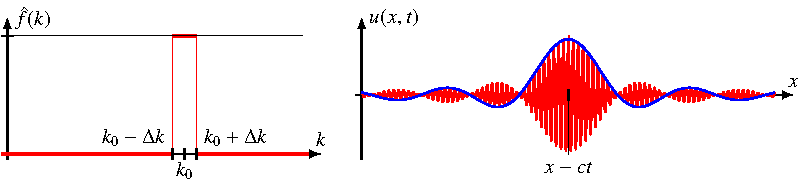
\includegraphics{chapters/7/wellenpaket.pdf}
\caption{Berechnung eines Wellenpaketes aus Wellen mit Wellenzahlen
zwischen $k_0-\Delta k$ und $k_0+\Delta k$.
\label{rossby:wellenpaket}}
\end{figure}
Wir betrachten ein Wellenpaket, welches als Überlagerung mit der
Amplitudenfunktion
\[
\hat f(k)
=
\begin{cases}
1&\qquad |k-k_0| < \Delta k\\
0&\qquad\text{sonst}
\end{cases}
\]
wie in Abbildung~\ref{rossby:wellenpaket} entsteht.
Die Überlagerung $u(x,t)$ gemäss~\eqref{rossby:komplexeueberlagerung}
kann man jetzt vereinfachen:
\[
u(x,t)
=
\operatorname{Re}
\int_{-\infty}^\infty \hat f(k)\,e^{i(kx-\omega(k)t)}\,dk
=
\operatorname{Re}
\int_{k_0-\Delta k}^{k_0+\Delta k} e^{i(kx-\omega(k)t)}\,dk,
\]
allerdings muss dazu $\omega(k)$ bekannt sein.

Falls $\omega(k)=ck$ gilt, falls also jede der elementaren Wellen
$\cos(kx-\omega t)$ die gleiche
Ausbreitungsgeschwindigkeit $c$ hat, können wir $u(x,t)$ explizit
ausrechnen:
\begin{align*}
u(x,t)
&=
\operatorname{Re}
\int_{k_0-\Delta k}^{k_0+\Delta k}
e^{i(kx-\omega(k)t)}\,dk
=
\operatorname{Re}
\int_{k_0-\Delta k}^{k_0+\Delta k}
e^{ik(x-ct)}\,dk
\\
&=
\operatorname{Re}
\biggl[
\frac{e^{ik(x-ct)}}{i(x-ct)}
\biggr]_{k_0-\Delta k}^{k_0+\Delta k}
=
\operatorname{Re}
\biggl(
\frac{e^{i(k_0+\Delta k)(x-ct)}}{i(x-ct)}
-
\frac{e^{i(k_0-\Delta k)(x-ct)}}{i(x-ct)}
\biggr)
\\
&=
\operatorname{Re}\frac{2}{x-ct}
e^{ik_0(x-ct)}\frac{e^{i\Delta k(x-ct)}-e^{i\Delta k(x-ct)}}{2i}
\\
&=
\operatorname{Re}\frac{2}{x-ct}
e^{ik_0(x-ct)}
\sin (\Delta k(x-ct))
=
2\cos k_0(x-ct) \frac{\sin \Delta k(x-ct)}{x-ct}
\end{align*}
Dies ist eine schnell schwankende Funktion mit Wellenzahl $k_0$, rot
dargestellt in Abbildung~\ref{rossby:wellenpaket} rechts, moduliert
mit der langsam schwankenden Funktion $\sin\Delta k(x-ct)/(x-ct)$,
dargestellt in der selben Abbildung in blau.
Der Schwerpunkt des Paketes befindet sich bei der $x$-Koordinaten $x-ct$,
er wandert also mit Geschwindigkeit $c$ nach rechts.

\subsubsection{Gruppengeschwindigkeit}
\index{Gruppengeschwindigkeit}%
Bisher haben wir angenommen, dass die Frequenz und die Wellenzahl proportional
sind, dass also $\omega(k)=ck$.
Die Untersuchungen zu den Rossby-Wellen hat gezeigt, dass dies nicht
zutreffen muss.
Wir müssen die Rechnung also mit einem Modell wiederholen, in dem die
Frequenz $\omega(k)$ nicht einfach nur proportional zu $k$ ist.
Für kleines $\Delta k$ genügt eine lineare Approximation der
Abhängigkeit von $\omega(k)$ von $k$, wir setzen daher
\begin{equation}
\omega(k)
=
\omega(k_0) + (k-k_0)\omega_1
=
\omega_0 + (k-k_0)\omega_1
\qquad
\text{mit}
\quad
\omega_1 = \frac{d}{dk}\omega(k_0) = \omega'(k_0).
\end{equation}
Wir berechnen wieder $u(x,t)$ wie folgt:
\begin{align*}
u(x,t)
&=
\operatorname{Re}
\int_{k_0-\Delta k}^{k_0+\Delta k}
e^{i(kx-\omega(k)t}\,dk
=
\operatorname{Re}
\int_{k_0-\Delta k}^{k_0+\Delta k}
e^{i(kx-\omega_0t -\omega_1(k-k_0)t)}
\,dk
\\
&=
\operatorname{Re}
\int_{k_0-\Delta k}^{k_0+\Delta k}
e^{i(k(x-\omega_1 t)-\omega_0t +\omega_1k_0t)}
\,dk
=
\operatorname{Re}
\int_{k_0-\Delta k}^{k_0+\Delta k}
e^{ik(x-\omega_1 t)}
e^{i(\omega_1k_0-\omega_0)t}
\,dk
\\
&=
\operatorname{Re}
e^{i(\omega_1k_0-\omega_0)t}
\biggl[
\frac{e^{ik(x-\omega_1 t)}}{i(x-\omega_1 t)}
\biggr]_{k_0-\Delta k}^{k_0+\Delta k}
=
\operatorname{Re}
2e^{i(\omega_1k_0-\omega_0)t}
\frac{
e^{i(k_0+\Delta k)(x-\omega_1 t)}
-
e^{i(k_0-\Delta k)(x-\omega_1 t)}
}{2i(x-\omega_1 t)}
\\
&=
\operatorname{Re}
\frac{2e^{i(\omega_1k_0-\omega_0)t}e^{i(k_0(x-\omega_1 t))}}{x-\omega_1 t}
\frac{
e^{i\Delta k(x-\omega_1 t)}
-
e^{-i\Delta k(x-\omega_1 t)}
}{2i}
=
\operatorname{Re}
2e^{i(\omega_1k_0-\omega_0+k_0(x-\omega_1 t))}
\frac{\sin \Delta k(x-\omega_1t)}{x-\omega_1 t}
\\
&=
\operatorname{Re}
2e^{i(k_0x-\omega_0t)}\,
\frac{\sin \Delta k(x-\omega_1t)}{x-\omega_1 t}
=
2\cos(k_0x-\omega_0t)
\frac{\sin \Delta k(x-\omega_1t)}{x-\omega_1 t}.
\end{align*}
Wiederum erhalten wir eine kurze Welle mit Frequenz
$\omega_0$ und Wellenzahl $k_0$, die moduliert wird mit der langsam
schwankenden Funktion
\begin{equation}
\frac{\sin\Delta k(x-\omega_1t)}{x-\omega_1 t}.
\label{rossby:gruppe}
\end{equation}
Das Maximum der Funktion~\eqref{rossby:gruppe}
befindet sich bei $x=\omega_1 t$, wandert also mit der
Geschwindigkeit $\omega_1$ nach rechts.

Die soeben durchgeführte Berechnung zeigt also, dass Wellenpakete
mit der Geschwindigkeit 
\[
c_g=\frac{d\omega(k)}{dk},
\]
der sogenannten {\em Gruppengeschwindigkeit}, wandern.
\index{Gruppengeschwindigkeit}%
Der Energietransport durch Wellenpakete erfolgt offenbar nicht
mit der Ausbreitungsgeschwindigkeit $c=\omega/k$, sondern mit der
Gruppengeschwindigkeit.

\subsection{Energietransport durch Rossby-Wellen\label{rossby:transport}}
Aus der Dispersionsrelation~\eqref{rossby:dispersion}
für die Rossby-Wellen können wir jetzt die Gruppengeschwindigkeit
für parallel zum Äquator sich bewegende Wellenpakete
durch Ableiten nach $k$ bestimmen.
Die Gruppengeschwindigkeit ist
\begin{equation}
c_g
=
\frac{d}{dk}\omega(k)
=
U-\beta
\frac{k^2+l^2-k\cdot 2k}{(k^2+l^2)^2}
=
U-\beta
\frac{l^2-k^2}{(k^2+l^2)^2}
\end{equation}
Je nach der relativen Grösse von $k$ und $l$ kann die
Gruppengeschwindigkeit sowohl grösser als auch kleiner sein als die
mittlere Geschwindigkeit $U$ in der Zone.
Rossby-Wellen können also je nach Wellenzahl sowohl nach Westen wie
auch nach Osten laufen.








%
% verzoegert.tex
%
% (c) 2018 Prof Dr Andreas Müller, Hochschule Rapperswil
%
\section{Verzögertes Oszillator-Modell\label{section:dde-nino}}
In den Kelvin- und Rossby-Wellen haben wir Mechanismen kennengelernt,
die Energietransport entlang des Äquators innerhalb der vorherrschenden
Strömung sowohl in östlicher wie auch in westlicher Richtung ermöglichen.
Entscheidend für die Dynamik dieses Energietransports ist die Zeit,
die eine Welle benötigt, um den Pazifik zu durchqueren.
Sei $\tau_K$ die Zeit, die eine Kelvin-Welle braucht, um den Pazifik
zu durchqueren, und $\tau_R$ die entsprechende Zeit für eine Rossby-Welle.

\rhead{Verzögertes Oszillator-Modell}
Wir versuchen jetzt, ein für die Temperaturanomalie $T(t)$ im östlichen
Pazifik aufzustellen, die diese Mechanismen berücksichtigt.
Ohne einen Transportmechanismus würde die Temperaturanomalie einfach
zerfallen, was beschrieben werden kann mit einer Differentialgleichung
der Form
\[
\frac{d}{dt}T(t)
=
-cT(t),
\]
mit einer Konstanten $c$.

\def\halb{\bgroup\textstyle\frac12\egroup}

Die Diskussionen über die dem El~Niño-Phänomen zugrunde liegenden
Mechanismen haben wir gesehen, dass die Thermoklinenanomalie im
zentralen Pazifik eine Auswirkung auf Temperatur\-anomalie $T(t)$ hat.
Eine Thermoklinenanomalie $h_0(t)$ am Äquator wandert als
Kelvin-Welle in der Zeit $\frac12\tau_K$ in den Ostpazifik.
Eine Thermoklinenanomalie $h_1(t)$ nördlich oder südlich des Äquators
kann als Rossby-Welle nach Westen wandern, am Westrand des Pazifik
reflektiert werden und als Kelvin-Welle in den Ostpazifik zurückkehren.
Dazu ist die Zeit $\frac12\tau_R+\tau_K$ nötig.
Dies lässt sich mit der Differentialgleichung
\begin{equation}
\frac{d}{dt}T(t)
=
-cT(t) + a_0h_0(t-\halb\tau_K) + b_0h_1(t-(\halb\tau_R+\tau_K))
\label{elninodde:1}
\end{equation}
erreichen.

Nun scheint es aber auch einen Zusammenhang zwischen der Temperaturanomalie
im Ostpazifik und den Thermoklinenanomalien im zentralen Pazifik zu geben.
Im einfachsten Fall kännen wir diesen Zusammenhang linear modellieren,
also 
\[
h_0(t-\halb\tau_K)
\sim
T(t-\halb\tau_K),
\qquad
\text{und}
\qquad
h_1(t-(\halb\tau_R+\tau_K))
\sim
T(t-(\halb\tau_R+\tau_K)).
\]
Eingesetzt in die Differentialgleichung~\eqref{elninodde:1} wird dabei zu
\begin{equation}
\frac{d}{dt}T(t)
=
-cT(t) + aT(t-\halb\tau_K) + bT(t-(\halb\tau_R+\tau_K))
\label{elninodde:2}
\end{equation}
Die Ableitung $\dot T(t)$ hängt also nicht nur von der Temperaturanomalie
zur Zeit $t$ ab, sondern auch von den Temperaturanomalien zu den
früheren Zeitpunkten $t-\halb\tau_K$ und $t-(\halb\tau_R-\tau_K)$.
Man nennt
\eqref{elninodde:2}
eine verzögerte Differentialgleichung.
\index{verzögerte Differentialgleichung}%

Die Theorie der linearen, verzögerten Differentialgleichungen wie 
\eqref{elninodde:2} zeigt, dass sie ähnlich wie gewöhnliche linear
Differentialgleichungen erster Ordnung Lösungen haben, die exponentiell
schnell zerfallen oder exponentiell anwachsen.
Daher können wir nicht erwarten, dass \eqref{elninodde:2} das El~Niño-Phänomen
adäquat beschreiben kann.
Um das exponentielle Anwachsen zu verhindern, braucht es einen zusätzlichen
Term, der dem Anwachsen von $T(t)$ überproportional entgegenwirkt.
Zum Beispiel könnte dies man mit einem Term der Form $-\varepsilon T(t)^3$
erreichen.
Die verzögerte Differentialgleichung ist dann
\begin{equation}
\frac{d}{dt}T(t)
=
-cT(t) + aT(t-\halb\tau_K) + bT(t-(\halb\tau_R+\tau_K))
-\varepsilon T(t)^3.
\label{elninodde:3}
\end{equation}
Ein andere Möglichkeit, ein ähnliches Ziel zu erreichen, wird in Kapitel
\ref{chapter:planeten} dargestellt.

In Kapitel~\ref{chapter:verzoegert} wird das Verhalten der Lösungen
solcher verzögerter Differentialgleichungen etwas mehr im Detail
diskutiert und es wird gezeigt, dass sie tatsächlich wesentliche
Aspekte des El~Niño-Phänomens adäquat wiedergeben können.










%
% kelvin.tex
%
% (c) 2018 Prof Dr Andreas Müller, Hochschule Rapperswil
%
\section{Kelvin-Wellen\label{section:elnino:kelvin}}
\rhead{Kelvin-Wellen}
In diesem Abschnitt soll die Ausbreitung von Anomalien in der Höhe
der Meeresoberfläche in der Nähe des Äquators studiert werden.

\subsection{Kelvin-Wellen\label{subsection:kelvin}}
\index{Kelvin-Wellen}
In der einfachsten Form führt ein Tiefdruckgebiet über dem zentralen
Pazifik dazu, dass die Meeresoberfläche über die Normalhöhe ansteigt.
Wenn sich das Tiefdruckgebiet auffüllt und die Druckkraft zur Aufrechterhaltung
dieser Anomalie wegfällt, wird dieser ``Wasserberg'' zerfallen.
Mit Hilfe der Gleichungen der Strömungsdynamik sollte sich die Ausbreitung
dieser Wellen beschreiben lassen.

Da die Anfangsbedingungen symmetrisch bezüglich einer Spiegelung an
der Äquatorebene sind, dürfen wir annehmen, dass auch die resultierende
Strömung diese Symmetrie hat.
In unmittelbarer Nähe des Äquators brauchen wir die Krümmung der
Erdoberfläche nicht zu berücksichtigen, und können daher mit einem
$x$-$y$-Koordinatensystem arbeiten, in dem $x$ die Richtung entlang des
Äquators und $y$ die Richtung entlang der Längenkreise ist (siehe auch
die Beschreibung der $\beta$-Ebene auf
Seite~\pageref{skript:betaplane:definition}).
\index{$\beta$-Ebene}%
Die Strömungsgeschwindigkeitskomponenten nennen wir $u$ entlang des
Äquators und $v$ entlang der Längenkreise.
Die Anomalie der Höhe der Meeresoberfläche bezeichnen wir mit $h(x,y)$.

\subsection{Bewegungsgleichung für Kelvin-Wellen}
Die zeitliche Änderung der Geschwindigkeit, also die Beschleunigung,
ist nach dem zweiten Newtonschen Gesetz proportional zu den Kräften.
Die Schwerkraft versucht, den Wasserberg abzubauen.
Wasser wird in diejenige Richtung beschleunigt, in die die Höhe $h(x,y)$
abnimmt.
Ausserdem wirkt die Coriolis-Kraft, die die Strömung auf der Nordhalbkugel
nach rechts ablenkt und auf der Südhalbkugel nach links.
So erhalten wir die Bewegungsgleichungen
\begin{equation}
\begin{aligned}
\frac{\partial u}{\partial t}
&=
\phantom{-}
fv - g\frac{\partial h}{\partial x}
\\
\frac{\partial v}{\partial t}
&=
-fu - g\frac{\partial h}{\partial y}.
\end{aligned}
\label{elnino:kelvin:newton}
\end{equation}
Dies ist ein System von zwei partiellen Differentialgleichung für 
drei unbekannte Funktionen $h$, $u$ und $v$, es ist also mindestens
noch eine weitere Gleichung nötig, damit das Problem überhaupt gelöst
werden kann.

Abfliessendes Wasser reduziert die Höhenanomalie.
Die Kontinuitätsgleichung~\eqref{skript:kontinuitaetsgleichung}
besagt, dass die Abnahme der Höhenanomalie $h$ proportional ist zur
Divergenz des Geschwindigkeitsfeldes.
Die fehlende Differentialgleichung ist daher
\begin{equation}
\frac{\partial h}{\partial t}
=
-H\biggl(
\frac{\partial u}{\partial x} + \frac{\partial v}{\partial y}
\biggr).
\label{elnino:kelvin:kont}
\end{equation}
Gesucht ist jetzt also eine Lösung der Differentialgleichungen
\eqref{elnino:kelvin:newton} und \eqref{elnino:kelvin:kont}.

\subsection{Wellengleichung}
Wir interessieren uns nur für eine Lösung in unmittelbarer Nähe des
Äquators und dürfen daher annehmen, dass sich das Wasser nicht
entlang der Längenkreise bewegt, dass also $v=0$ gilt.
Die Differentialgleichungen
\eqref{elnino:kelvin:newton} und \eqref{elnino:kelvin:kont}
vereinfachen sich damit zu
\begin{align}
\frac{\partial u}{\partial t}
&=
\phantom{-fu}
 - g\frac{\partial h}{\partial x}
\label{kelvin:naeherung:1}
\\
0
&=
-fu - g\frac{\partial h}{\partial y}
\label{kelvin:naeherung:2}
\\
\frac{\partial h}{\partial t}
&=
-H
\frac{\partial u}{\partial x}
\label{kelvin:naeherung:3}
\end{align}
Wir suchen nach einem Wellenphänomen entlang des Äquators, dafür
brauchen wir eine Wellengleichung in den Variablen $t$ und $x$,
die in den Gleichungen \eqref{kelvin:naeherung:1} nach
\eqref{kelvin:naeherung:3} vorkommen.
Aus diesen beiden Gleichungen sollte sich eine Wellengleichung
gewinnen lassen.

Indem wir \eqref{kelvin:naeherung:1} nach $x$ und 
\eqref{kelvin:naeherung:3} nach $t$ ableiten, erhalten wir
\begin{equation}
\left.
\begin{aligned}
\frac{\partial^2 u}{\partial x\,\partial t}
&=
-g\frac{\partial^2h}{\partial x^2}
\\
\frac{\partial^2 h}{\partial t^2}
&=
-H\frac{\partial^2 u}{\partial t\,\partial x}
\end{aligned}
\;
\right\}
\quad
\Rightarrow
\quad
\frac{\partial^2 h}{\partial t^2}
=
gH\frac{\partial^2 h}{\partial x^2}
\label{kelvin:wellengleichung}
\end{equation}
Dies ist die gesuchte Wellengleichung für eine Welle mit
Ausbreitungsgeschwindigkeit $c=\sqrt{gH}$.
Im nächsten Abschnitt bestimmen wir ihre Lösungen.

\subsection{Approximative Lösung der Wellengleichung}
Bis jetzt wurde die zweite Gleichung~\eqref{kelvin:naeherung:2}
nicht verwendet, es wurde eigentlich nur das Verhalten der Welle auf
dem Äquator modelliert.
Da wir jetzt aber wissen, dass mindestens entlang des Äquators die Lösung
eine Welle mit Ausbreitungsgeschwindigkeit $c=\sqrt{gH}$ ist, können
wir versuchen, auch die $y$-Abhängigkeit zu modellieren.

\subsubsection{Dispersionsrelation}
Eine in $x$-Richtung laufende Welle mit Wellenzahl $k$ kann beschrieben werden
als $\cos(kx-\omega t)$.
Die Wellenzahl $k$ ist positiv für eine nach Osten laufende Welle und negativ
für eine nach Westen laufende Welle.
Überall dort, wo $kx-\omega t=0$ ist, befindet sich ein Wellenberg,
die Position dieses Maximums ist also
\[
x=\frac{\omega}{k}\cdot t,
\]
es bewegt sich also mit der Geschwindigkeit $c=\omega/k$.
Dies ist die sogenannte {\em Phasengeschwindigkeit}.
\index{Phasengeschwindigkeit}%

Wir dürfen allerdings nicht davon ausgehen, dass das Verhältnis $\omega/k$
konstant ist, Wellen mit verschiedenen Frequenzen können sich durchaus
mit verschiedenen Geschwindigkeiten ausbreiten.
Ein Glasprisma ist in der Lage, Licht in seine verschiedene Farben
mit verschiedenen Ausbreitungsgeschwindigkeiten im Glas aufzufächern. 
Dieses Phänomen heisst {\em Dispersion} und äussert sich in einem
\index{Dispersion}%
funktionalen Zusammenhang
\[
\omega = \omega(k)
\]
zwischen Wellenzahl $k$ und Frequenz $\omega$, einer {\em Dispersionsrelation}.
\index{Dispersionsrelation}%

Wir suchen also eine Lösung des Gleichungssystems
\eqref{kelvin:naeherung:1}--\eqref{kelvin:naeherung:3}
in der Form
\[
h_k(t,x,y) = \gamma(y)\cdot \cos(kx-\omega t)
\]
zu finden.
Die Funktion $\gamma(y)$ beschreibt das Profil des ``Wasserberges'' 
in der Nähe des Äquators, wir nehmen daher an, dass $\gamma(y)$ für grosse
Werte von $y$ rasch abnimmt.

Einsetzen des Lösungsansatzes $h_k(t,x,y)$ in die
Gleichung~\eqref{kelvin:wellengleichung} liefert
\begin{equation}
\left.
\begin{aligned}
\frac{\partial^2 h_k}{\partial t^2}
&=
- \omega^2 \gamma(y) \cos(kx-\omega t)
=
-\omega^2 h_k(t,x,y)
\\
\frac{\partial^2 h_k}{\partial x^2}
&=
-
k^2
\gamma(y)
\cos (kx-\omega t)
=
-k^2 h_k(t,x,y)
\end{aligned}
\;\right\}
\quad
\Rightarrow
\quad
\omega^2=gHk^2
\quad\text{oder}\quad
\biggl|
\frac{\omega}{k}\biggr|
=\sqrt{gH}=c
\end{equation}
Aus dieser Dispersionsrelation
liest man ab, dass die Phasengeschwindigkeit einer solchen
Welle unabhängig ist von der Frequenz.

\subsubsection{$y$-Abhängigkeit}
Bis jetzt haben wir die Gleichung~\eqref{kelvin:naeherung:2} nicht
verwendet.
Sie erlaubt, $u$ zu berechnen, es gilt
\[
u=-\frac{g}{f}\,\frac{\partial h}{\partial y}
\qquad
\text{oder für $h_k$}
\qquad
u_k=-\frac{g}{f} \gamma'(y) \sin(kx-\omega t).
\]
Setzt man dies in \eqref{kelvin:naeherung:3} ein, erhält man
\begin{equation}
\left.
\begin{aligned}
\frac{\partial h_k}{\partial t}
&=
-\omega
\gamma(y) \cos(kx-\omega t)
\\
\frac{\partial u_k}{\partial x}
&=
k \frac{g}{f}\gamma'(y) \cos(kx-\omega t)
\end{aligned}
\;\right\}
\qquad\Rightarrow\qquad
-\omega
\gamma(y) \cos(kx-\omega t)
=
-H
k \frac{g}{f}\gamma'(y) \cos(kx-\omega t).
\end{equation}
Nach Kürzen gemeinsamer Faktoren und Umstellen folgt
\begin{equation}
\gamma'(y)
=
\gamma(y) \frac{f}{gH}\frac{\omega}{k}
=
\pm
\frac{f}{c} \gamma(y).
\label{kelvin:gamma:dgl1}
\end{equation}
Das Vorzeichen in \eqref{kelvin:gamma:dgl1} hängt vom Vorzeichen der
Wellenzahl $k$ ab, das obere Vorzeichen steht für eine nach Osten
laufende Welle.

Die Coriolis-Kraft $f$ verschwindet am Äquator, in erster Näherung
ist sie proportional zu $y$, wir schreiben daher $f=\beta y$.
Die Differentialgleichung~\eqref{kelvin:gamma:dgl1} wird damit zu
\begin{equation}
\gamma'(y)
=
\pm
\frac{\beta}{c} 
y\gamma(y).
\label{kelvin:gamma:dgl2}
\end{equation}

Für zunehmende $y$ muss $\gamma$ abnehmen, es muss also $\gamma'(y)<0$ sein
für genügend grosse $y$.
Dies ist aber nur möglich für das negative Vorzeichen, und damit nur
für eine nach Osten laufende Welle.
Im Folgenden konzentrieren wir uns daher auf das negative Zeichen
in \eqref{kelvin:gamma:dgl2}.

Um eine Lösung von \eqref{kelvin:gamma:dgl2} zu finden, teilen wir
durch $\gamma(y)$
und verwenden, dass $\gamma'(y)/\gamma(y)$ die Ableitung des
Logarithmus ist:
\begin{equation}
\frac{\gamma'(y)}{\gamma(y)}
=
\frac{d}{dy}\log \gamma(y) = -\frac{\beta}{c} y
\qquad\Rightarrow\qquad
\log\gamma(y) = -\frac{\beta}{2c}y^2
\qquad\Rightarrow\qquad
\gamma(y) = \exp\biggl(
- \frac{\beta}{2c}y^2
\biggr)
\end{equation}
Das $y$-Profil der Welle ist also eine Gauss-Funktion.
Die Zone, in der sich eine Kelvin-Welle ausbreiten kann, 
wird schmaler, wenn $\beta$ grösser wird, wenn also die 
Rotationsgeschwindigkeit des Planeten grösser wird.
Sie wird kleiner, wenn $c=\sqrt{gH}$ grösser wird, also
bei grösserer Gravitation.


%
% rossby.tex
%
% (c) 2018 Prof Dr Andreas Müller, Hochschule Rapperswil
%

\section{Rossby-Wellen\label{section:elnino:rossby}}
\rhead{Rossby-Wellen}
In der Untersuchung der Kelvin-Wellen haben wir angenommen, dass die
Geschwindigkeit $v$ entlang der Längenkreise verschwindet.
Die Strömung wird aber im Allgemeinen nicht parallel zum Äquator sein.
Wir beobachten zum Beispiel, dass die Westwindströmung 
zwischen verschiedenen geographischen Breiten mäandriert.
Woher kommt diese Wellenbewegung?
\index{Rossby-Wellen}%

\subsection{Zirkulation\label{subsection:rossby:zirkulation}}
Aus der Diskussion der globalen Zirkulation in
Kapitel~\ref{chapter:wetter und klima} wissen wir, dass die
Strömung in Äquatornähe dominiert wird durch eine mittlere
konstante Strömung mit Geschwindigkeit $U$ in Ost-West-Richtung.
Wir suchen daher eine Beschreibung der Abweichungen von dieser
mittleren Strömung.
Unter Verwendung der gleichen Notation wie im
Abschnitt~\ref{section:elnino:kelvin} schreiben wir daher
\[
u'=U+u,\qquad v'=v\qquad\text{mit $u,v\ll U$}.
\]
Die Geschwindigkeitskomponenten $u$ und $v$ sind die Anomalien relativ
zur vorherrschenden mittleren Strömung.

Wir nehmen im Folgenden wieder an, dass die Strömung quellenfrei ist.
Dann lässt sich wie früher gezeigt die Strömung mit einer
Strömungsfunktion $\psi$ als
\begin{equation}
u=-\frac{\partial \psi}{\partial y},\qquad
v=\frac{\partial\psi}{\partial x}
\label{skript:rossby:geschwindigkeit}
\end{equation}
beschreiben.

Die gesuchten Wellen sollen Mäander-Form der Strömung erklären,
also Änderungen der Strömungsrichtungen, die natürlich mit
Änderungen des Drehimpulses einhergehen.
Die Drehimpulsdichte in der Strömung ist gegeben durch die Zirkulation
\[
\zeta
=
\frac{\partial v}{\partial x} - \frac{\partial u}{\partial y}
=
\Delta \psi.
\]
Da der Drehimpuls erhalten ist, muss die Zirkulation in einem
Luftpaket abnehmen, wenn es sich auf der Nordhalbkubel nach Norden
bewegt.
Die Quelle dieser Zirkulationsänderung ist die Erddrehung und damit
die Corioliskraft $f$ und der mathematische Ausdruck der Drehimpulserhaltung
ist die Erhaltung der Grösse $\zeta+f$.

\subsection{Bewegungsgleichung\label{subsection:rossby:bewegungsgleichung}}
Die Grösse $\zeta+f$ ist erhalten, daher muss ihre zeitliche Ableitung
\[
\frac{d(\zeta f)}{dt}=0
\]
verschwinden.
Die Coriolis-Kraft
$f$ hängt nur von $y$ ab, aber die Funktion $\zeta$ hängt von allen
drei Variablen $t$, $x$ und $y$ ab.
Wir berechnen die Ableitung mit Hilfe der Kettenregel:
\begin{align*}
0
=
\frac{d(\zeta+f)}{dt}
&=
\frac{\partial\zeta}{\partial t}
+
\frac{\partial\zeta}{\partial x}\cdot \frac{dx}{dt}
+
\frac{\partial(\zeta+f)}{\partial y}\cdot\frac{dy}{dt}
\\
&\simeq
\frac{\partial\zeta}{\partial t}
+
(U+u)\frac{\partial\zeta}{\partial x}
+
v\biggl(\frac{\partial\zeta}{\partial y} + \frac{\partial f}{\partial y}\biggr).
\end{align*}
Da $u\ll U$ ist, können wir in erster Näherung $u$ im zweiten Term 
vernachlässigen.
Und da $\partial\zeta/\partial y$ ebenfalls sehr klein ist, können
wir dies im letzten Term im Vergleich zu $\partial f/\partial y$
vernachlässigen.
Schliesslich können wir wie in Abschnitt~\ref{section:elnino:kelvin}
die $\beta$-Ebenen-Approximation verwenden und $\partial f/\partial y$
durch $\beta$ ersetzen.
Schliesslich können wir wieder mit \eqref{skript:rossby:geschwindigkeit}
$v$ als Ableitung von $\psi$ nach $x$ ausdrücken.
Wir erhalten so
\[
0
=
\frac{\partial\zeta}{\partial t}
+
U\frac{\partial\zeta}{\partial x}
+
\beta\frac{\partial\psi}{\partial x}
\]
als Bewegungsgleichung.

Indem wir $\zeta=\Delta \psi$ schreiben, erhalten wir so die 
Bewegungsgleichung
\begin{equation}
\frac{\partial\Delta\psi}{\partial t}
+
U\frac{\partial\Delta\psi}{\partial x}
+
\beta\frac{\partial\psi}{\partial x}
=
0.
\label{rossby:gleichung}
\end{equation}


\subsection{Wellenlösungen\label{subsection:rossby:loesungen}}
Gesucht sind Lösungen der Gleichung~\eqref{rossby:gleichung}
in Form kleiner Abweichungen.
Wir erwarten Wellenlösungen und schreiben sie daher in der Form
\begin{equation}
\psi_{kl}(t,x,y)
=
\cos(kx+ly-\omega t).
\label{rossby:ebenewelle}
\end{equation}
Die Ableitungen, die wir für die Bewegungsgleichung
\eqref{rossby:gleichung} benötigen, sind
\begin{align*}
\frac{\partial}{\partial t} \psi_{kl}(t,x,y)
&=
\omega \sin(kx+ly-\omega t)
\\
\frac{\partial}{\partial x} \psi_{kl}(t,x,y)
&=
-k
\sin(kx+ly-\omega t)
\\
\Delta\psi_{kl}
&=
-(k^2+l^2)\cos(kx+ly-\omega t)=-(k^2+l^2)\psi_{kl}(t,x,y).
\end{align*}
Setzen wir dies in die Differentialgleichung
\eqref{rossby:gleichung}
ein, erhalten wir 
\begin{align*}
0
&=
-
\omega(k^2+l^2) 
\sin(kx+ly-\omega t)
+
Uk(k^2+l^2)
\sin(kx+ly-\omega t)
-
\beta k
\sin(kx+ly-\omega t)
\\
&=
-\bigl((\omega-Uk)(k^2+l^2)+\beta k\bigr)
\sin(kx+ly-\omega t).
\end{align*}
Für eine Lösung muss also die Dispersionsrelation
\[
(\omega -Uk)(k^2+l^2) +\beta k=0
\]
gelten.
Aufgelöst nach $\omega$ ist dies
\begin{align}
\omega(k^2+l^2)
&=
Uk(k^2+l^2) -\beta k
\notag
\\
\Rightarrow\qquad
\omega
&=
Uk
-
\frac{\beta k}{k^2+l^2}.
\label{rossby:dispersion}
\end{align}
Eine Wellenlösung mit Wellenzahlen $k$ und $l$ hat daher 
die Ausbreitungsgeschwindigkeit 
\begin{equation}
c=\frac{\omega}{k} = U-\beta\frac{1}{k^2+l^2}
\label{rossby:phasengeschwindigkeit}
\end{equation}
entlang der $x$-Koordinate.
Da der Nenner immer positiv ist, ist $c$ kleiner als $U$, solche
Wellen können sich immer nur in West-Ost-Richtung ausbreiten.

\subsection{Gruppengeschwindigkeit}
Die Phasengeschwindigkeit~\eqref{rossby:phasengeschwindigkeit}
hilft uns nicht, die Dynamik des El Niño zu verstehen, da wir dazu
den Transport von Energie verstehen müssen.
Die ebenen Wellen der Form~\eqref{rossby:ebenewelle} beschreiben eine Welle,
die überall die gleiche Amplitude hat.
Ein Transport von potentieller Energie findet aber nur statt, wenn ein
``Wellenberg'' sich an einen anderen Ort bewegt.
Im Beispiel des ``Wasserberges'' in der Untersuchung zu den Kelvin-Wellen
wird potentielle Energie dadurch transportiert, dass das Wasser des Berges
abfliesst.
Wir müssen daher erst einen ``Wasserberg'' als Überlagerung von 
ebenen Wellen formulieren und dann die zeitliche Entwicklung dieser
Überlagerung studieren.

\subsubsection{Überlagerungen}
Wir gehen von einer eindimensionalen Situation aus und studieren
eine Überlagerung $u(x,t)$ von Wellen der Form $\cos(kx-\omega(k) t)$
mit verschiedenen Wellenzahlen $k$.
Mit der wellenzahlabhängigen Amplitude $\hat f(k)$, dem Spektrum
wie in Kapitel~\ref{chapter:fourier} studiert, lässt sich die
Überlagerung als
\begin{equation}
u(x,t)
=
\int_{-\infty}^\infty \hat f(k)\,\cos(kx-\omega(k)t)\,dk
\label{rossby:reelleueberlagerung}
\end{equation}
schreiben.
Die Bewegung eines solchen Wellenpaketes kann man zum Beispiel
dadurch studieren, dass man die Bewegung des Maximums dieses 
Wellenpaketes verfolgt.
\index{Wellenpaket}

Die Darstellung~\eqref{rossby:reelleueberlagerung} ist für diese
Untersuchung sehr unhandlich, die Rechnungen sind zu umständlich.
Wir schreiben die Wellen daher als Realteil einer komplexen
Welle $e^{i(kx-\omega(k)t)}$, also
\begin{equation}
u(x,t)
=
\operatorname{Re}
\int_{-\infty}^\infty \hat f(k)\,e^{i(kx-\omega(k)t)}\,dk.
\label{rossby:komplexeueberlagerung}
\end{equation}
Dabei lassen wir auch zu, dass $\hat{f}(k)$ komplexe Werte annimmt.

\subsubsection{Wellenpakete}
\begin{figure}
\centering
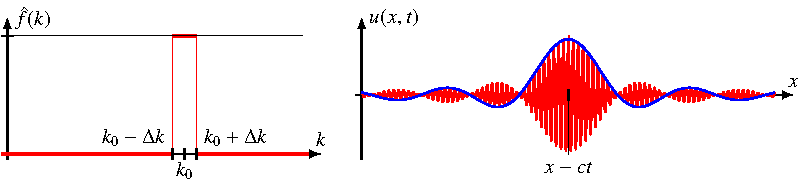
\includegraphics{chapters/7/wellenpaket.pdf}
\caption{Berechnung eines Wellenpaketes aus Wellen mit Wellenzahlen
zwischen $k_0-\Delta k$ und $k_0+\Delta k$.
\label{rossby:wellenpaket}}
\end{figure}
Wir betrachten ein Wellenpaket, welches als Überlagerung mit der
Amplitudenfunktion
\[
\hat f(k)
=
\begin{cases}
1&\qquad |k-k_0| < \Delta k\\
0&\qquad\text{sonst}
\end{cases}
\]
wie in Abbildung~\ref{rossby:wellenpaket} entsteht.
Die Überlagerung $u(x,t)$ gemäss~\eqref{rossby:komplexeueberlagerung}
kann man jetzt vereinfachen:
\[
u(x,t)
=
\operatorname{Re}
\int_{-\infty}^\infty \hat f(k)\,e^{i(kx-\omega(k)t)}\,dk
=
\operatorname{Re}
\int_{k_0-\Delta k}^{k_0+\Delta k} e^{i(kx-\omega(k)t)}\,dk,
\]
allerdings muss dazu $\omega(k)$ bekannt sein.

Falls $\omega(k)=ck$ gilt, falls also jede der elementaren Wellen
$\cos(kx-\omega t)$ die gleiche
Ausbreitungsgeschwindigkeit $c$ hat, können wir $u(x,t)$ explizit
ausrechnen:
\begin{align*}
u(x,t)
&=
\operatorname{Re}
\int_{k_0-\Delta k}^{k_0+\Delta k}
e^{i(kx-\omega(k)t)}\,dk
=
\operatorname{Re}
\int_{k_0-\Delta k}^{k_0+\Delta k}
e^{ik(x-ct)}\,dk
\\
&=
\operatorname{Re}
\biggl[
\frac{e^{ik(x-ct)}}{i(x-ct)}
\biggr]_{k_0-\Delta k}^{k_0+\Delta k}
=
\operatorname{Re}
\biggl(
\frac{e^{i(k_0+\Delta k)(x-ct)}}{i(x-ct)}
-
\frac{e^{i(k_0-\Delta k)(x-ct)}}{i(x-ct)}
\biggr)
\\
&=
\operatorname{Re}\frac{2}{x-ct}
e^{ik_0(x-ct)}\frac{e^{i\Delta k(x-ct)}-e^{i\Delta k(x-ct)}}{2i}
\\
&=
\operatorname{Re}\frac{2}{x-ct}
e^{ik_0(x-ct)}
\sin (\Delta k(x-ct))
=
2\cos k_0(x-ct) \frac{\sin \Delta k(x-ct)}{x-ct}
\end{align*}
Dies ist eine schnell schwankende Funktion mit Wellenzahl $k_0$, rot
dargestellt in Abbildung~\ref{rossby:wellenpaket} rechts, moduliert
mit der langsam schwankenden Funktion $\sin\Delta k(x-ct)/(x-ct)$,
dargestellt in der selben Abbildung in blau.
Der Schwerpunkt des Paketes befindet sich bei der $x$-Koordinaten $x-ct$,
er wandert also mit Geschwindigkeit $c$ nach rechts.

\subsubsection{Gruppengeschwindigkeit}
\index{Gruppengeschwindigkeit}%
Bisher haben wir angenommen, dass die Frequenz und die Wellenzahl proportional
sind, dass also $\omega(k)=ck$.
Die Untersuchungen zu den Rossby-Wellen hat gezeigt, dass dies nicht
zutreffen muss.
Wir müssen die Rechnung also mit einem Modell wiederholen, in dem die
Frequenz $\omega(k)$ nicht einfach nur proportional zu $k$ ist.
Für kleines $\Delta k$ genügt eine lineare Approximation der
Abhängigkeit von $\omega(k)$ von $k$, wir setzen daher
\begin{equation}
\omega(k)
=
\omega(k_0) + (k-k_0)\omega_1
=
\omega_0 + (k-k_0)\omega_1
\qquad
\text{mit}
\quad
\omega_1 = \frac{d}{dk}\omega(k_0) = \omega'(k_0).
\end{equation}
Wir berechnen wieder $u(x,t)$ wie folgt:
\begin{align*}
u(x,t)
&=
\operatorname{Re}
\int_{k_0-\Delta k}^{k_0+\Delta k}
e^{i(kx-\omega(k)t}\,dk
=
\operatorname{Re}
\int_{k_0-\Delta k}^{k_0+\Delta k}
e^{i(kx-\omega_0t -\omega_1(k-k_0)t)}
\,dk
\\
&=
\operatorname{Re}
\int_{k_0-\Delta k}^{k_0+\Delta k}
e^{i(k(x-\omega_1 t)-\omega_0t +\omega_1k_0t)}
\,dk
=
\operatorname{Re}
\int_{k_0-\Delta k}^{k_0+\Delta k}
e^{ik(x-\omega_1 t)}
e^{i(\omega_1k_0-\omega_0)t}
\,dk
\\
&=
\operatorname{Re}
e^{i(\omega_1k_0-\omega_0)t}
\biggl[
\frac{e^{ik(x-\omega_1 t)}}{i(x-\omega_1 t)}
\biggr]_{k_0-\Delta k}^{k_0+\Delta k}
=
\operatorname{Re}
2e^{i(\omega_1k_0-\omega_0)t}
\frac{
e^{i(k_0+\Delta k)(x-\omega_1 t)}
-
e^{i(k_0-\Delta k)(x-\omega_1 t)}
}{2i(x-\omega_1 t)}
\\
&=
\operatorname{Re}
\frac{2e^{i(\omega_1k_0-\omega_0)t}e^{i(k_0(x-\omega_1 t))}}{x-\omega_1 t}
\frac{
e^{i\Delta k(x-\omega_1 t)}
-
e^{-i\Delta k(x-\omega_1 t)}
}{2i}
=
\operatorname{Re}
2e^{i(\omega_1k_0-\omega_0+k_0(x-\omega_1 t))}
\frac{\sin \Delta k(x-\omega_1t)}{x-\omega_1 t}
\\
&=
\operatorname{Re}
2e^{i(k_0x-\omega_0t)}\,
\frac{\sin \Delta k(x-\omega_1t)}{x-\omega_1 t}
=
2\cos(k_0x-\omega_0t)
\frac{\sin \Delta k(x-\omega_1t)}{x-\omega_1 t}.
\end{align*}
Wiederum erhalten wir eine kurze Welle mit Frequenz
$\omega_0$ und Wellenzahl $k_0$, die moduliert wird mit der langsam
schwankenden Funktion
\begin{equation}
\frac{\sin\Delta k(x-\omega_1t)}{x-\omega_1 t}.
\label{rossby:gruppe}
\end{equation}
Das Maximum der Funktion~\eqref{rossby:gruppe}
befindet sich bei $x=\omega_1 t$, wandert also mit der
Geschwindigkeit $\omega_1$ nach rechts.

Die soeben durchgeführte Berechnung zeigt also, dass Wellenpakete
mit der Geschwindigkeit 
\[
c_g=\frac{d\omega(k)}{dk},
\]
der sogenannten {\em Gruppengeschwindigkeit}, wandern.
\index{Gruppengeschwindigkeit}%
Der Energietransport durch Wellenpakete erfolgt offenbar nicht
mit der Ausbreitungsgeschwindigkeit $c=\omega/k$, sondern mit der
Gruppengeschwindigkeit.

\subsection{Energietransport durch Rossby-Wellen\label{rossby:transport}}
Aus der Dispersionsrelation~\eqref{rossby:dispersion}
für die Rossby-Wellen können wir jetzt die Gruppengeschwindigkeit
für parallel zum Äquator sich bewegende Wellenpakete
durch Ableiten nach $k$ bestimmen.
Die Gruppengeschwindigkeit ist
\begin{equation}
c_g
=
\frac{d}{dk}\omega(k)
=
U-\beta
\frac{k^2+l^2-k\cdot 2k}{(k^2+l^2)^2}
=
U-\beta
\frac{l^2-k^2}{(k^2+l^2)^2}
\end{equation}
Je nach der relativen Grösse von $k$ und $l$ kann die
Gruppengeschwindigkeit sowohl grösser als auch kleiner sein als die
mittlere Geschwindigkeit $U$ in der Zone.
Rossby-Wellen können also je nach Wellenzahl sowohl nach Westen wie
auch nach Osten laufen.








%
% verzoegert.tex
%
% (c) 2018 Prof Dr Andreas Müller, Hochschule Rapperswil
%
\section{Verzögertes Oszillator-Modell\label{section:dde-nino}}
In den Kelvin- und Rossby-Wellen haben wir Mechanismen kennengelernt,
die Energietransport entlang des Äquators innerhalb der vorherrschenden
Strömung sowohl in östlicher wie auch in westlicher Richtung ermöglichen.
Entscheidend für die Dynamik dieses Energietransports ist die Zeit,
die eine Welle benötigt, um den Pazifik zu durchqueren.
Sei $\tau_K$ die Zeit, die eine Kelvin-Welle braucht, um den Pazifik
zu durchqueren, und $\tau_R$ die entsprechende Zeit für eine Rossby-Welle.

\rhead{Verzögertes Oszillator-Modell}
Wir versuchen jetzt, ein für die Temperaturanomalie $T(t)$ im östlichen
Pazifik aufzustellen, die diese Mechanismen berücksichtigt.
Ohne einen Transportmechanismus würde die Temperaturanomalie einfach
zerfallen, was beschrieben werden kann mit einer Differentialgleichung
der Form
\[
\frac{d}{dt}T(t)
=
-cT(t),
\]
mit einer Konstanten $c$.

\def\halb{\bgroup\textstyle\frac12\egroup}

Die Diskussionen über die dem El~Niño-Phänomen zugrunde liegenden
Mechanismen haben wir gesehen, dass die Thermoklinenanomalie im
zentralen Pazifik eine Auswirkung auf Temperatur\-anomalie $T(t)$ hat.
Eine Thermoklinenanomalie $h_0(t)$ am Äquator wandert als
Kelvin-Welle in der Zeit $\frac12\tau_K$ in den Ostpazifik.
Eine Thermoklinenanomalie $h_1(t)$ nördlich oder südlich des Äquators
kann als Rossby-Welle nach Westen wandern, am Westrand des Pazifik
reflektiert werden und als Kelvin-Welle in den Ostpazifik zurückkehren.
Dazu ist die Zeit $\frac12\tau_R+\tau_K$ nötig.
Dies lässt sich mit der Differentialgleichung
\begin{equation}
\frac{d}{dt}T(t)
=
-cT(t) + a_0h_0(t-\halb\tau_K) + b_0h_1(t-(\halb\tau_R+\tau_K))
\label{elninodde:1}
\end{equation}
erreichen.

Nun scheint es aber auch einen Zusammenhang zwischen der Temperaturanomalie
im Ostpazifik und den Thermoklinenanomalien im zentralen Pazifik zu geben.
Im einfachsten Fall kännen wir diesen Zusammenhang linear modellieren,
also 
\[
h_0(t-\halb\tau_K)
\sim
T(t-\halb\tau_K),
\qquad
\text{und}
\qquad
h_1(t-(\halb\tau_R+\tau_K))
\sim
T(t-(\halb\tau_R+\tau_K)).
\]
Eingesetzt in die Differentialgleichung~\eqref{elninodde:1} wird dabei zu
\begin{equation}
\frac{d}{dt}T(t)
=
-cT(t) + aT(t-\halb\tau_K) + bT(t-(\halb\tau_R+\tau_K))
\label{elninodde:2}
\end{equation}
Die Ableitung $\dot T(t)$ hängt also nicht nur von der Temperaturanomalie
zur Zeit $t$ ab, sondern auch von den Temperaturanomalien zu den
früheren Zeitpunkten $t-\halb\tau_K$ und $t-(\halb\tau_R-\tau_K)$.
Man nennt
\eqref{elninodde:2}
eine verzögerte Differentialgleichung.
\index{verzögerte Differentialgleichung}%

Die Theorie der linearen, verzögerten Differentialgleichungen wie 
\eqref{elninodde:2} zeigt, dass sie ähnlich wie gewöhnliche linear
Differentialgleichungen erster Ordnung Lösungen haben, die exponentiell
schnell zerfallen oder exponentiell anwachsen.
Daher können wir nicht erwarten, dass \eqref{elninodde:2} das El~Niño-Phänomen
adäquat beschreiben kann.
Um das exponentielle Anwachsen zu verhindern, braucht es einen zusätzlichen
Term, der dem Anwachsen von $T(t)$ überproportional entgegenwirkt.
Zum Beispiel könnte dies man mit einem Term der Form $-\varepsilon T(t)^3$
erreichen.
Die verzögerte Differentialgleichung ist dann
\begin{equation}
\frac{d}{dt}T(t)
=
-cT(t) + aT(t-\halb\tau_K) + bT(t-(\halb\tau_R+\tau_K))
-\varepsilon T(t)^3.
\label{elninodde:3}
\end{equation}
Ein andere Möglichkeit, ein ähnliches Ziel zu erreichen, wird in Kapitel
\ref{chapter:planeten} dargestellt.

In Kapitel~\ref{chapter:verzoegert} wird das Verhalten der Lösungen
solcher verzögerter Differentialgleichungen etwas mehr im Detail
diskutiert und es wird gezeigt, dass sie tatsächlich wesentliche
Aspekte des El~Niño-Phänomens adäquat wiedergeben können.









